\section{Extended current evidence and planned sensitivity analyses}
\label{sec:supp-results}

\subsection{Current evidence inventory}

The table below is an execution-oriented view of the current results and their required replacement artifacts. It is not a final statistical table.

\begingroup
\footnotesize
\setlength{\tabcolsep}{3pt}
\begin{longtable}{p{0.07\textwidth} p{0.22\textwidth} p{0.27\textwidth} p{0.30\textwidth}}
\caption{Analysis stages, primary estimands, and stage gates.}\label{tab:analysis-plan}\\
\toprule
Stage & Workstream & Primary output & Continue/downgrade rule \\
\midrule
\endfirsthead
\toprule
Stage & Workstream & Primary output & Continue/downgrade rule \\
\midrule
\endhead
00 & Preflight and source inventory & Data, label, code, and output hashes; schema audit & Fatal only for corrupted or uninterpretable canonical inputs \\
01 & Identity and geometry repair & Immutable site key; canonical mapping; regression tests & Must prove no spatial-site overwrite \\
02 & Label and timing contract & Original/adjudicated timing views; review panels & Continue with original timing while decisions remain pending \\
03 & Raw-to-pipeline trace atlas & Complete trace/metric inventory for every occurrence & Missing mandatory trace or untracked unit blocks dependent analysis \\
04 & Acquisition QC & Noise, saturation, drift, motion, field and optional-video reports & Optional videos may be absent; canonical QC is mandatory \\
05 & Scalar observability & Variance components, ICCs, rank stability, burst sensitivity & Singular models downgrade to fixed/rank-based summaries \\
06 & Spatial specificity & Radial profiles, matched controls, equivalence tests & Claims are downgraded if control matching or margins fail \\
07 & Functional and tensor analysis & Shared, site, burst and residual temporal components & Run only after completeness and held-out stability gates \\
08 & Measurement phenotype & Recoverability and failure-mode models & Clusters remain exploratory; continuous effects are primary \\
09 & Bounded annotation & Blinded packet and local precision--recall & Nonblocking until completed reviewer labels return \\
10 & Frozen representation panel & Utility, fidelity, burden and failure decomposition & No feature expansion; retain negative/equivalence results \\
11 & Manuscript export & Macros, tables, figures and source maps & Every numerical claim must resolve to a validated source \\
12 & Release validation & Reproducible package and aggregate decisions & Release fails if provisional or unresolved mandatory fields remain \\
\bottomrule
\end{longtable}
\endgroup


\subsection{Burst-specific sensitivity}

The protected output will report all primary scalar and trace metrics for each burst separately, with burst~2 highlighted as prespecified timing-uncertain. Required displays include:
\begin{itemize}
  \item event-aligned Raw, annulus, residual, difference, and ICA population traces by burst;
  \item native-amplitude distributions and robust SNR by burst;
  \item original versus proposed timing overlays for burst~2;
  \item each primary effect with and without burst~2;
  \item leave-one-burst-out effect estimates and component stability;
  \item a statement of whether the substantive conclusion changes under any sensitivity view.
\end{itemize}

\subsection{Identity sensitivity}

Until ROI~010/015 is adjudicated, the following result views are mandatory:
\begin{enumerate}
  \item original-site analysis with all \NCurrentOriginalSites{} coordinate-defined sites;
  \item provisional canonical analysis with \NCurrentCanonicalNeurons{} identities, retaining separate source traces;
  \item direct ROI~010-versus-ROI~015 trace and spatial comparison;
  \item a hypothetical merged summary only if a defensible consolidated mask or aggregation rule is specified;
  \item explicit identification of statistics that change under the merge view.
\end{enumerate}

\subsection{Provisional signature figures}

\ProvisionalFigure{0.94\linewidth}{provisional_signature_generalization.png}{Existing Raw-signature generalization summary. This figure is retained as a visual reference only and will be replaced by the repaired held-out site analysis.}{fig:supp-raw-signature}

\ProvisionalFigure{0.94\linewidth}{provisional_residual_signature_generalization.png}{Existing residual-signature generalization summary. The replacement will separate original-site geometry from canonical identity and include matched translated spatial controls.}{fig:supp-residual-signature}

\subsection{Detection-profile class centroids}

\begin{figure}[!htbp]
  \centering
  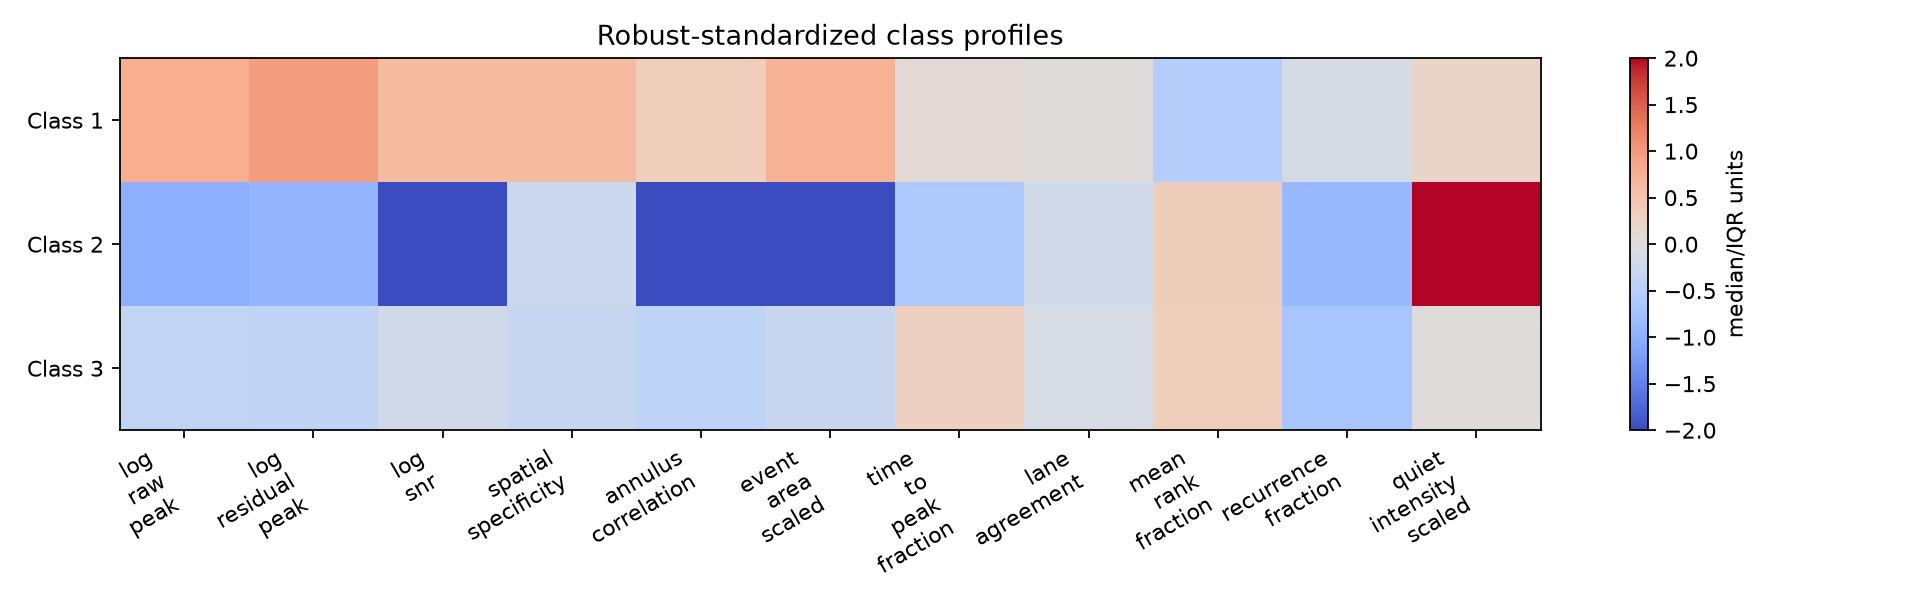
\includegraphics[width=0.98\linewidth]{figures/final/detection_class_profiles.png}
  \caption{Robust-standardized centroids of the three frozen detection-event classes. Signal and contextual measurements were standardized within burst; lane agreement, rank fraction, and recurrence used global robust scaling. Colors show median/IQR units and do not encode expert labels.}
  \label{fig:supp-detection-class-centroids}
\end{figure}

\subsection{Advanced post-freeze class profiling}

\begin{figure}[!htbp]
  \centering
  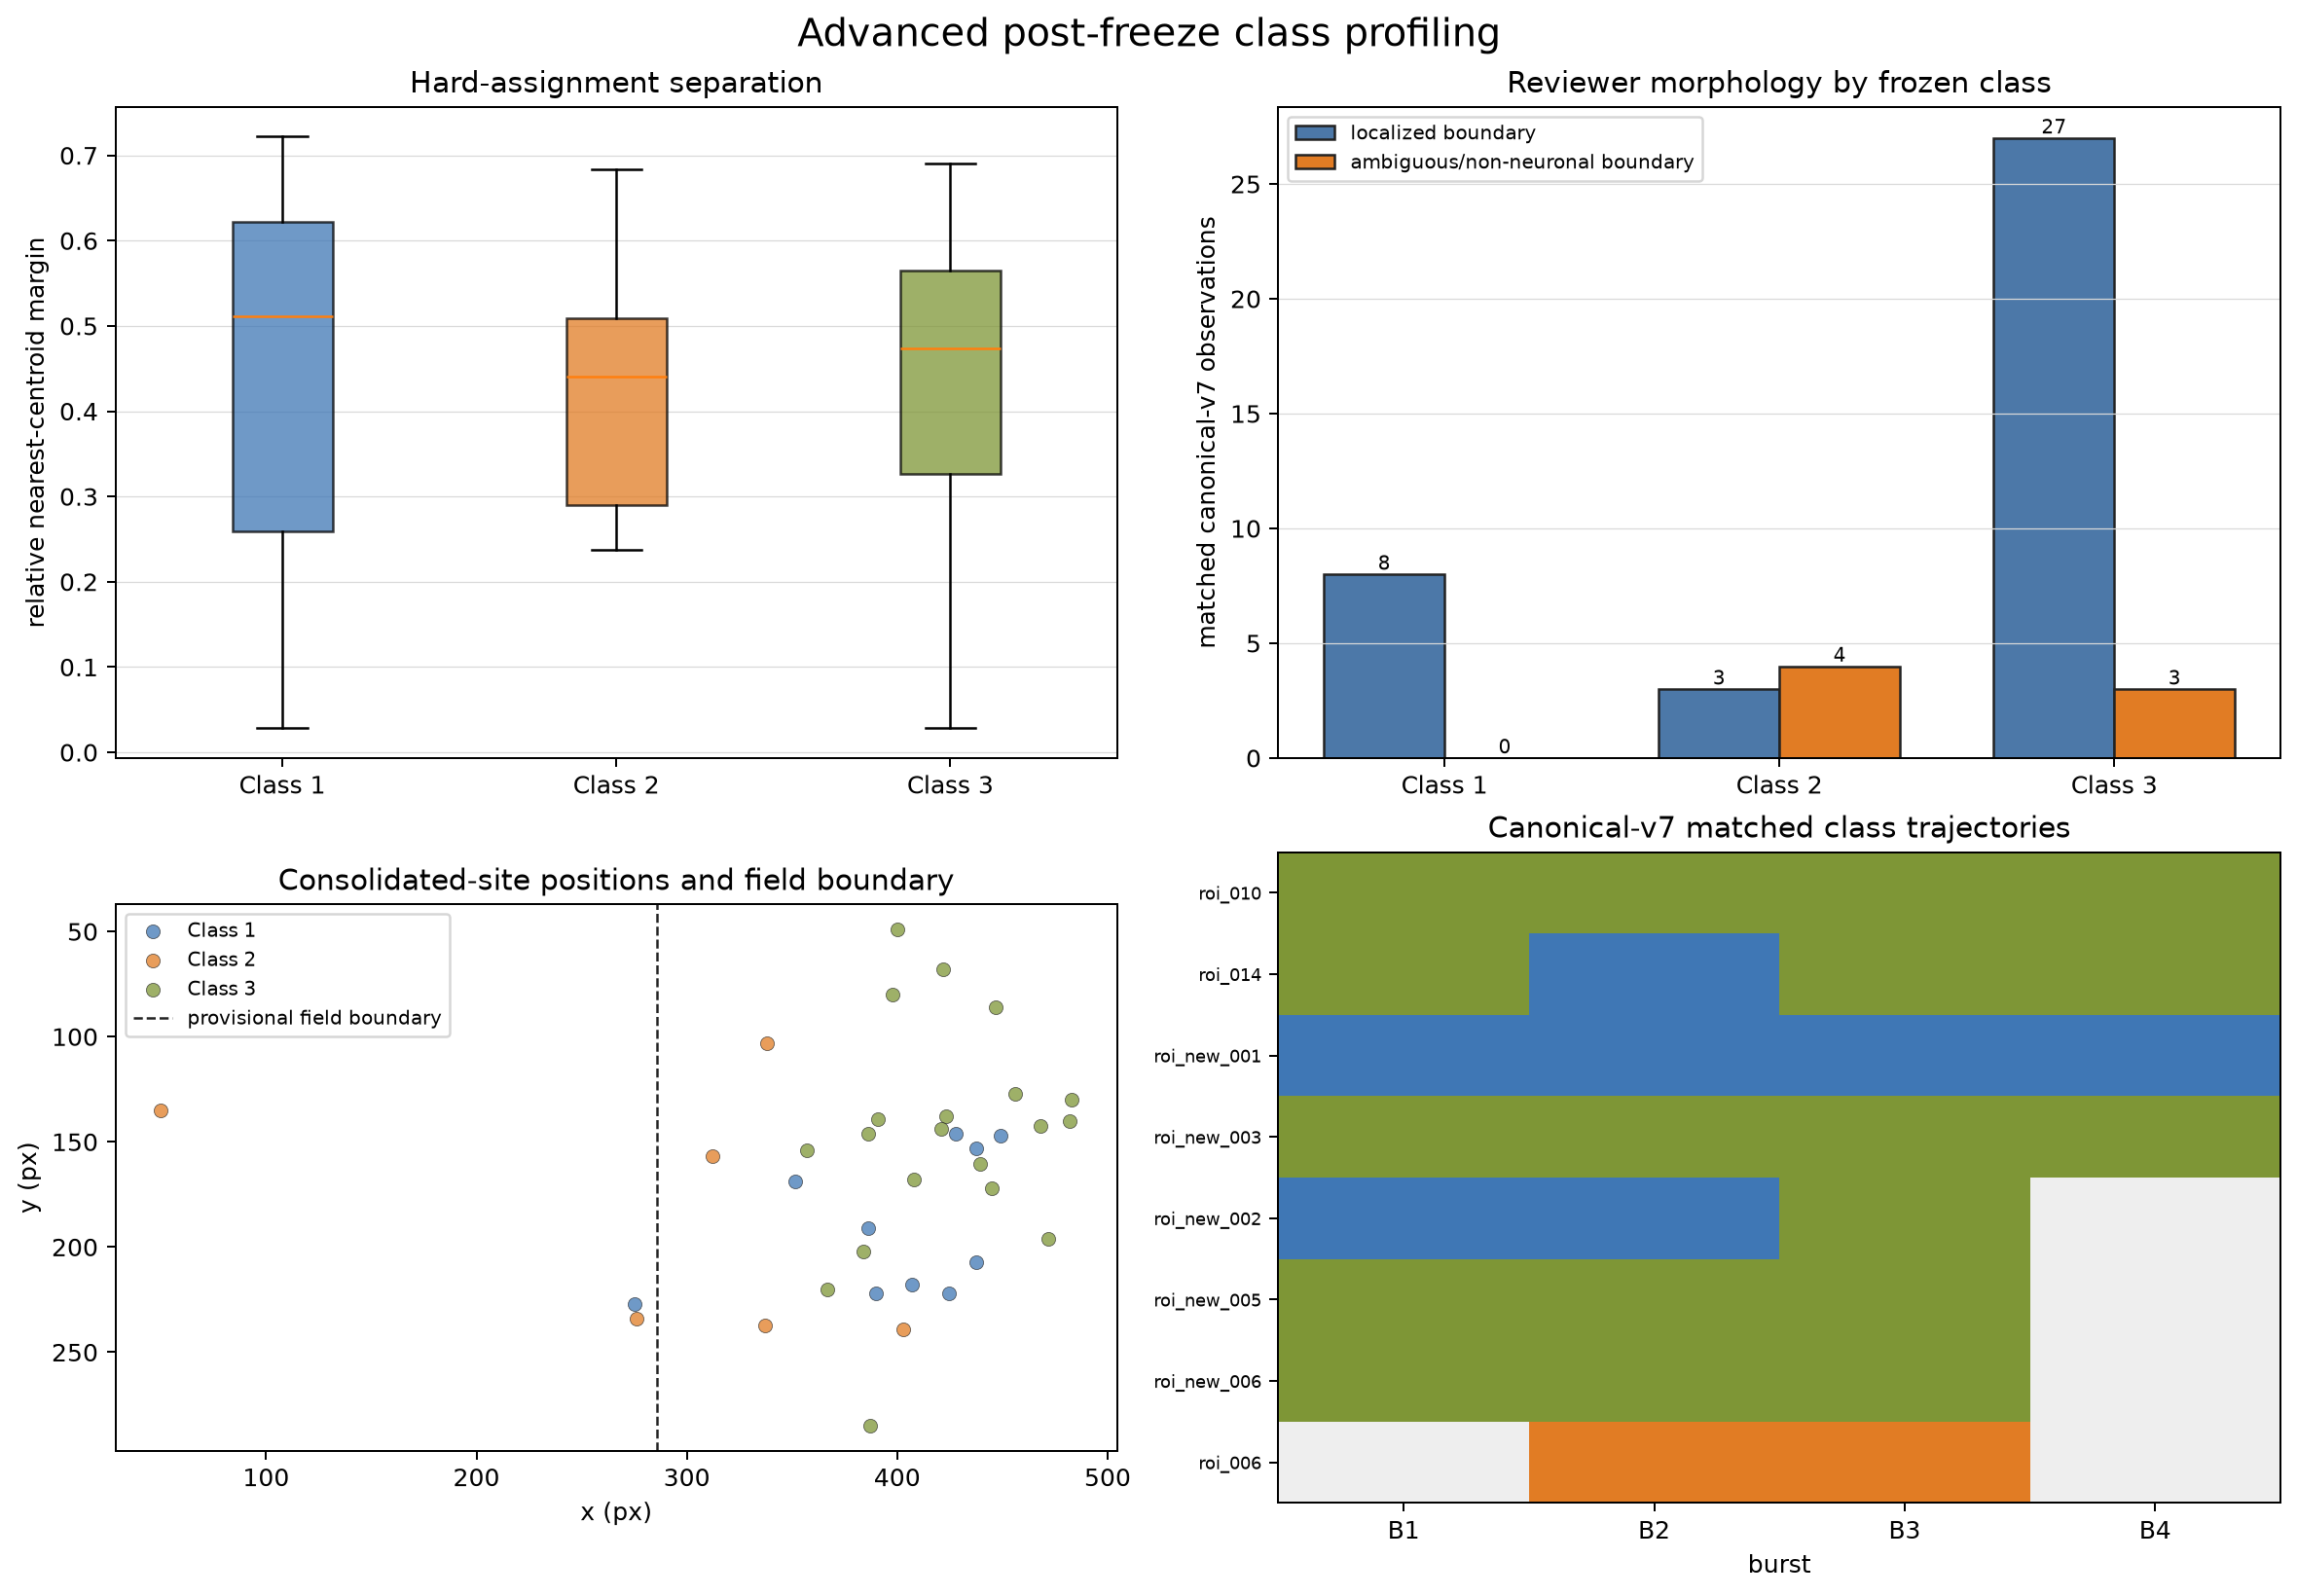
\includegraphics[width=0.98\linewidth]{figures/final/detection_class_advanced_extensions.png}
  \caption{Advanced detection-class extensions. The centroid margin measures relative hard-assignment separation and is not a posterior probability. Reviewer morphology and canonical trajectories use candidate-assisted canonical v7. Spatial positions are consolidated detection sites, so recurrent occurrences do not multiply the field comparison. Gray trajectory cells indicate no matched detection in that burst.}
  \label{fig:supp-detection-class-advanced}
\end{figure}

\subsection{Spatial ICA filter-level stability}

\begin{figure}[!htbp]
  \centering
  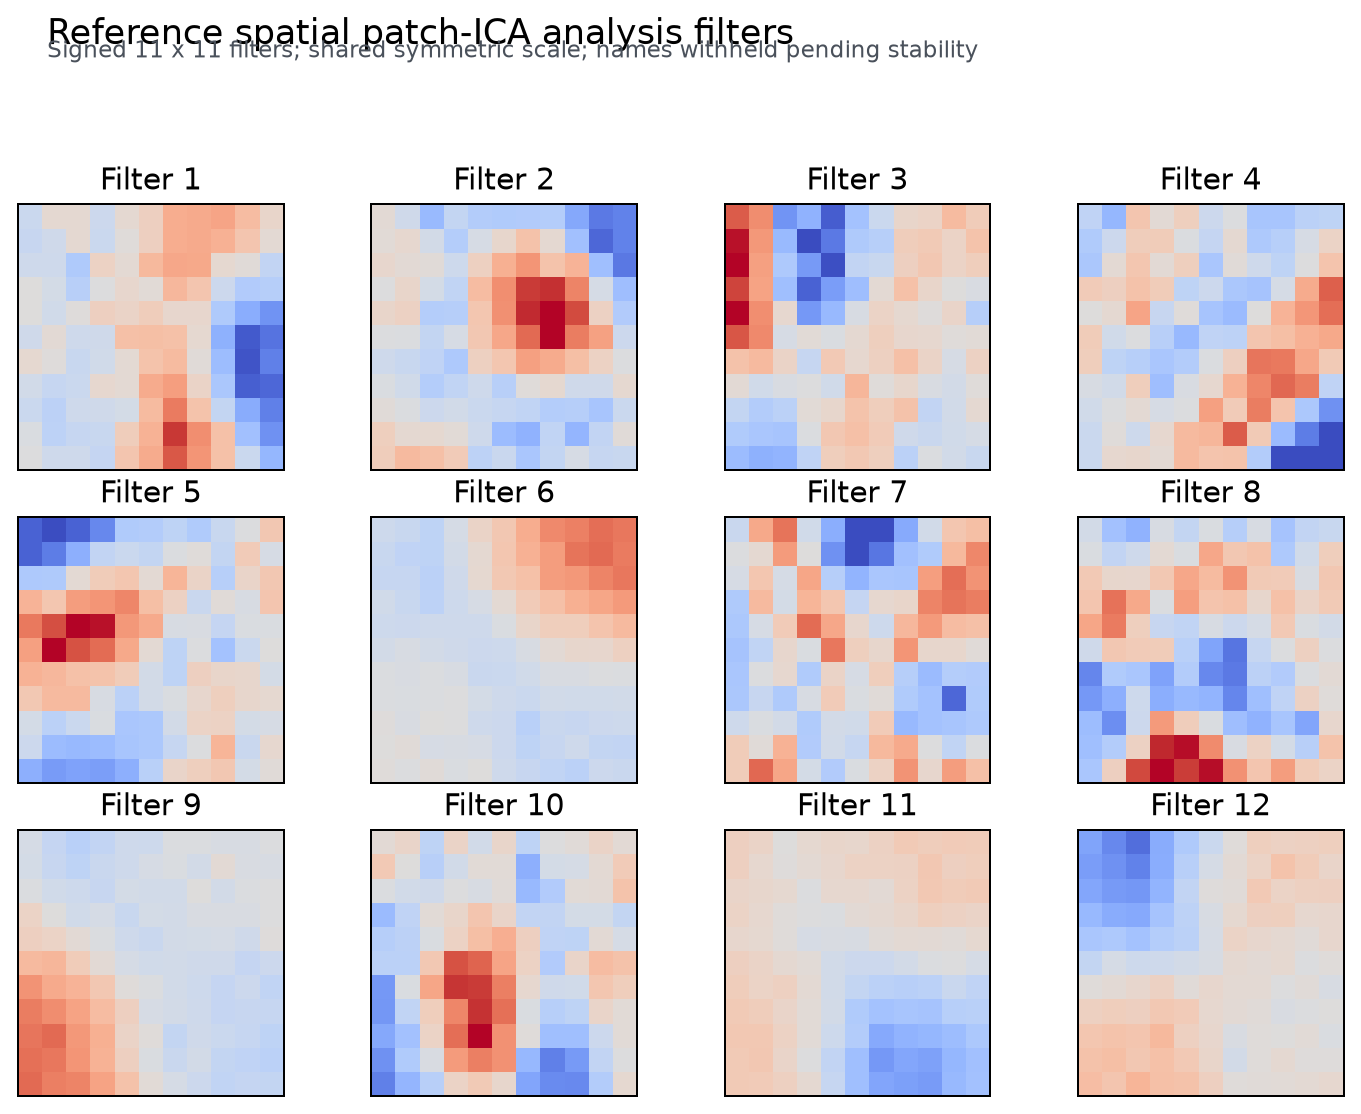
\includegraphics[width=0.98\linewidth]{figures/final/spatial_ica_filter_stability.png}
  \caption{Aligned spatial-ICA filters across random seeds and leave-one-burst-window-out refits. Subspaces were moderately similar, but individual aligned filters failed the prespecified interpretation threshold. The gallery is included to document why component-wise anatomical labels are prohibited even though the reconstructed output is stable.}
  \label{fig:supp-spatial-ica-filter-stability}
\end{figure}

\subsection{Negative and boundary results}

The complete-trace feature panel is an informative boundary result. At
confirmed centers, \FullTraceCarrierCeilingCount{} of \FullTraceOccurrences{}
carrier percentiles and \FullTraceLagCeilingCount{} lagged-recurrence
percentiles equal 1.0. No feature passes the incremental-over-carrier gate.
Consensus and multiscale persistence retain median available burst-pair site-rank
correlations of \FullTraceConsensusRepeatability{} and
\FullTracePersistenceRepeatability{}, but these are exploratory and require
independent-recording transfer. The complete machine-readable feature table is
packaged as \texttt{generated\_analysis/full\_trace\_feature\_panel\_v2/
feature\_summary.tsv}.

The manuscript will preserve scientifically valid negative results. In particular, the final report will state when:
\begin{itemize}
  \item a learned component is analytically equivalent to a simple operator;
  \item a repeatable event waveform is not spatially specific;
  \item a local residual has event amplitude but no stable shape;
  \item a functional or tensor model fails held-out stability;
  \item a representation improves known-positive recovery but materially degrades trace fidelity;
  \item an effect depends on burst~2, one field, one site, or one annotation choice;
  \item precision remains unidentified outside the bounded field.
\end{itemize}
These outcomes constrain future model design and should not be hidden by selective promotion.
